% !TeX spellcheck = en_US
\documentclass[sigconf,nonacm]{acmart}
\usepackage{listings}
\usepackage{subcaption}
\settopmatter{printacmref=false}
\pagestyle{empty}
\AtBeginDocument{%
  \providecommand\BibTeX{{%
    \normalfont B\kern-0.5em{\scshape i\kern-0.25em b}\kern-0.8em\TeX}}}
\copyrightyear{2020}
\acmYear{2020}
\setcopyright{rightsretained}
\begin{document}
\title{Deep Learning for Visual Computing}
\subtitle{Group 12, Exercise 2: Iterative Optimization and Parametric Models}
\author{SHU Yuting}
\email{e11931687@student.tuwien.ac.at}
\affiliation{Mat.Nr. 11931687}
\author{Helmuth BREITENFELLNER}
\email{helmuth.breitenfellner@student.tuwien.ac.at}
\affiliation{Mat.Nr. 08725866}
\begin{abstract}
In this assignment we have been experimenting with various optimizers,
to better understand their behavior for stochastic gradient
descent.
In addition we were developing a first deep neural network, using CNN,
for classifying cats and dogs from images.
Finally, to reduce issues from overfitting, we applied data augmentation,
regularization, early stopping and transfer learning, in various settings.
\end{abstract}
\keywords{Deep Learning, Linear Model, Visual Computing, Image Processing, PyTorch}
\maketitle
\section{Task description}
First we were asked to experiment with various functions and stochastic
gradient descent, in combination with different optimizers and
their hyperparameters.

Next task was to create a simple CNN, based on the framework already developed
for assignment 1.

Finally, we were requested to experiment with various techniques for avoiding overfitting.

\section{Gradient Descent}

\section{Network Architecture}

For this part of the exercise we were experimenting with three convolutional neural networks.
The first one, our baseline network, was based on the suggested network from the slides.

As a second network we used a simplified version, with only one ``block'', and for comparison
we also used a more complex one, with a third block.

\begin{figure}[ht]
\begin{subfigure}[c]{0.45\columnwidth}
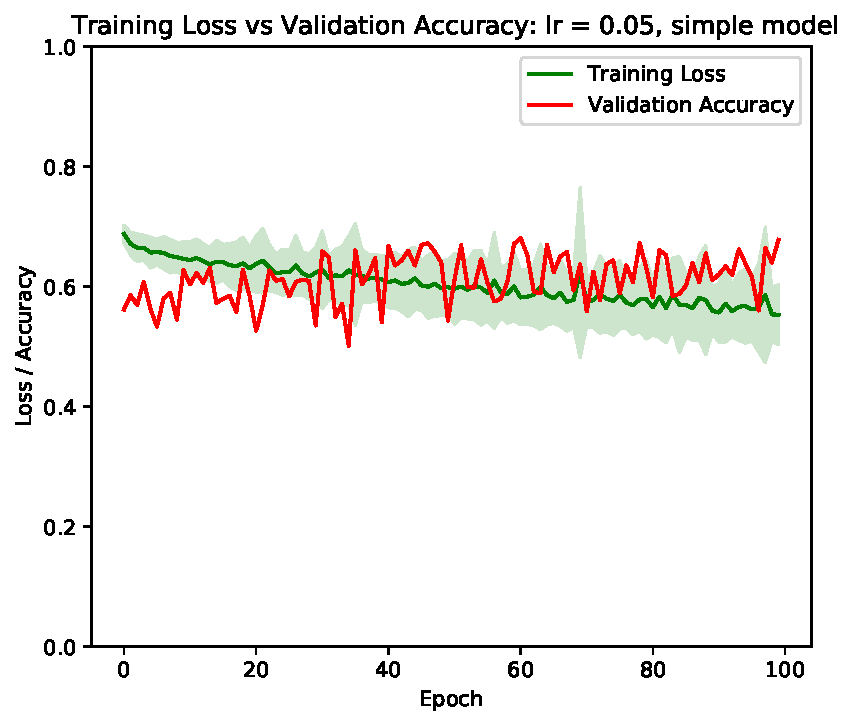
\includegraphics[width=\textwidth]{plot_simple_0.05.pdf}
\subcaption{Model too simple}
\end{subfigure}
\begin{subfigure}[c]{0.45\columnwidth}
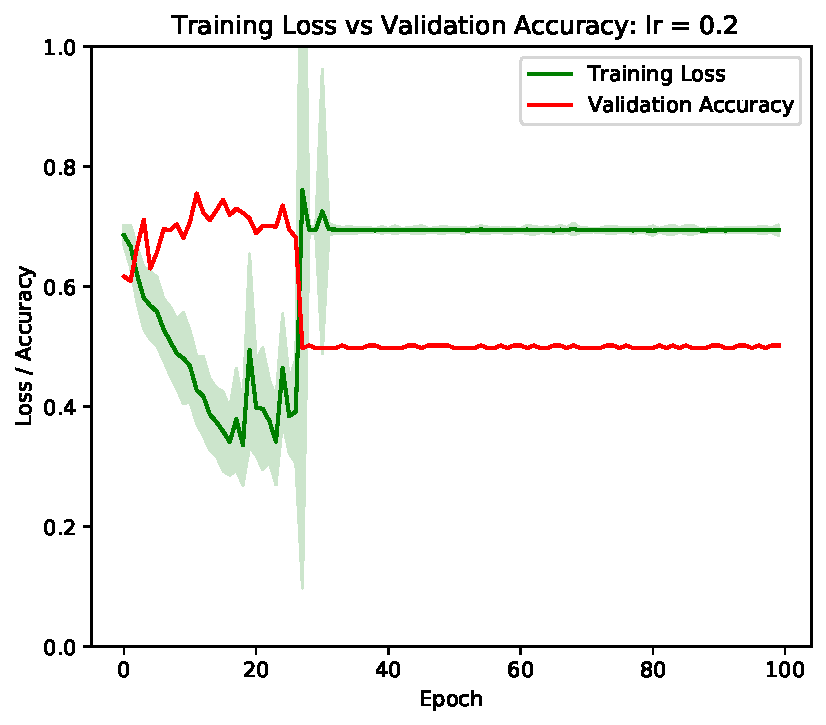
\includegraphics[width=\textwidth]{plot_0.2.pdf}
\subcaption{Learning rate too high}
\end{subfigure}
\caption{Diverging models}
\label{part2:diverging}
\end{figure}

\begin{figure}[ht]
\begin{subfigure}[c]{0.45\columnwidth}
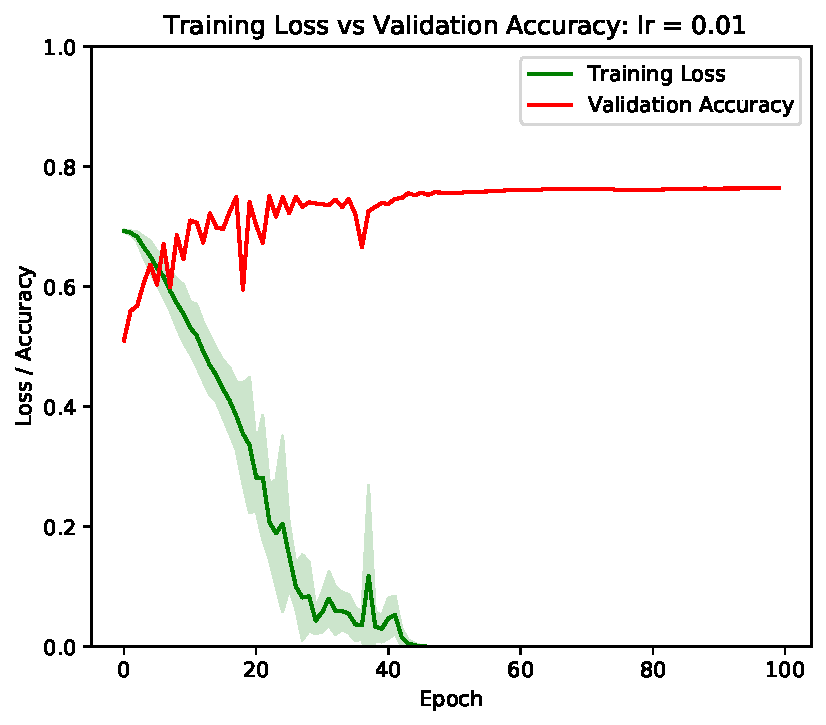
\includegraphics[width=\textwidth]{plot_0.01.pdf}
\subcaption{Regular model}
\end{subfigure}
\begin{subfigure}[c]{0.45\columnwidth}
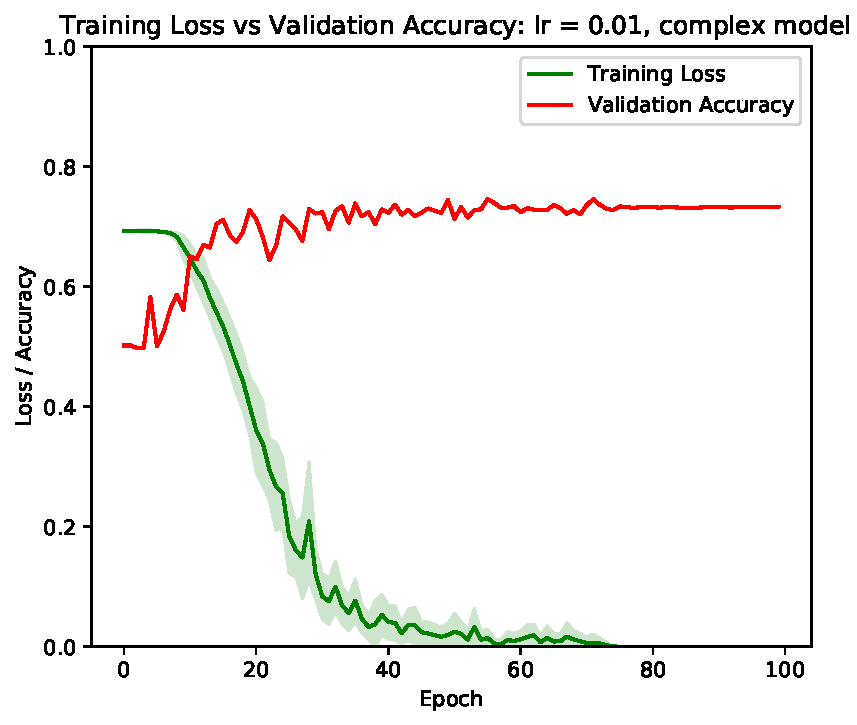
\includegraphics[width=\textwidth]{plot_complex_0.01.pdf}
\subcaption{Complex model}
\end{subfigure}
\caption{Converging models}
\label{part2:converging}
\end{figure}

\section{Avoiding of Overfitting}

\subsection{Data Augmentation}

\subsection{Regularization}
We tried weight decay wd = 0.01,
Dropout with p=0.25(without weight decay), p is the probability of an element to be zeroed,
Dropout with p=0.5(without weight decay)

\subsection{Early Stopping}
For regular model with learning rate as 0.01, with an early stop at epoch 38, we got a train loss as 0.017 and validation accuracy as 0.753.
\section{Transfer Learning}

\bibliographystyle{ACM-Reference-Format}
\bibliography{report}
\end{document}
